\documentclass[12pt]{article}

\usepackage{amsmath}
\usepackage{graphicx}

\title{A response to the review of the manuscript
``Seeq: a library for inexact DNA sequence matching''}
\date{}

\newenvironment{code}{\ttfamily}{\par}

\begin{document}
\maketitle
As the authors of the manuscript ``Seeq: a library for inexact
DNA sequence matching'', we would like to discuss some of the
ideas that were raised by the reviewers. We believe that
critical discussion, based on facts and arguments is fundamental
to the scientific process. We fully respect the decision of the
editor and of our peers, but we do not consider that we should
interrupt a fruitful discussion because the manuscript was
rejected. Please do not see in this letter a criticism of the
reviews, but simply a wish to touch upon questions that were
impossible to treat in a two page manuscript and to respond to
some of the points that were raised.

Since this is not a rebuttal, we will do our best to make it
informal and didactic. But before doing so, we would like to
thank the reviewers for a really outstanding work. We are
all for software quality and excellent science, we wish that every
tool were scrutinized with the same amout of care. We have learned
important lessons, and the suggestions will greatly help us improve
the software and the manuscript.

\section{The inception}

Our work on Seeq started with casual Internet browsing.
The first source was a seminal series of blog posts by Russ Cox [1]
explaining how and why he implemented the regular expression library
RE2. The key insight was that many modern regular expression engines
(including those of Perl and Python) have ``forgotten'' the
theory and many developers are unaware that lazy DFA-based
implementations outperform the alternatives.

The second source of inspiration was a blog post by Nick Johnson [2]
where he explains the use of Levenshtein automata in the problem of
approximate string query. In Fig.~\ref{generalities} we give some
generalities about Levenshtein automata, we also refer the interested
reader to the blog post of Nick Johnson, which is very clear and makes
a lively introduction to the subject, and to reference [3] for a
more comprehensive treatment.

\begin{figure}[!tpb]
\centerline{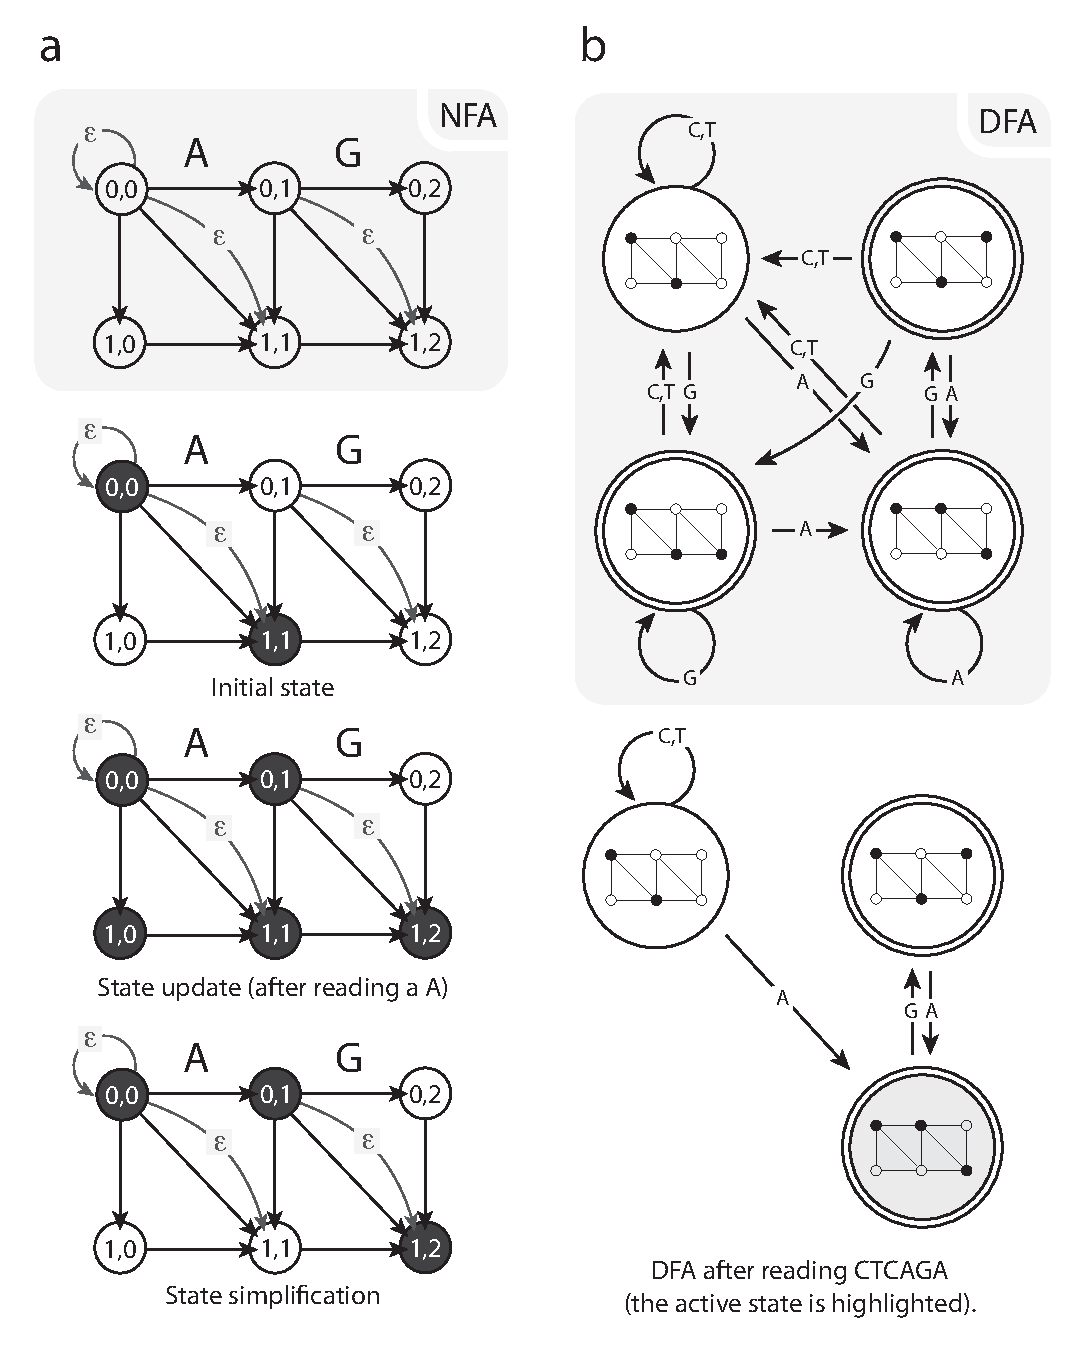
\includegraphics[scale=.6]{edit_matrix.pdf}}
\caption{Generalities on Levenshtein automata. a) Edit graph
of the string \texttt{GA} with 1 tolerated error. The edit graph
is a NFA with state transition as shown in the top panel. States
are labelled by two numbers indicating their number of errors and
their position relative to the search pattern. NFAs can be in
several active states (dark circles). The initial active states
of the NFA are as shown on the second panel. After reading
\texttt{A} from the input, the active states are updated as shown
on the third panel. The active states can be simplified by keeping
only the upper node on each column, as shown on the bottom panel.
b) DFA representation. Every NFA has a DFAs representation.
States of the DFA are sets of active states of the NFA. In a
lazy DFA, only the states required to process the input are present
(bottom panel).
}\label{generalities}
\end{figure}

When we had to identify oligos that we spiked in our sequencing
experiments for quantification purposes,
we gave a try to the Python implementation suggested
by Nick Johnson, which solved the problem (Illumina sequencing is
not indel-prone, but oligos synthesis is, which is why we needed
the Levenshtein distance). However, the Python prototype was rather
slow, and because it is a non lazy DFA, the memory footprint was too
high to allow more than two errors.

We connected the ideas of the two posts and we used the trick of
reversing the DFA to identify the position of the hit in the string
as suggested by Russ Cox. The first C implementation of Seeq gave
very good results and we decided to continue. We came across the
literature on lazy/partial DFAs later, but we knew from the outset
that the ideas were rather old  (for the record, lazy DFAs were
introduced by Alfred Aho in egrep in 1989).

So we agree with reviewer 2 that the algorithm is not novel, yet
we are curious where s/he finds any mention of lazy DFAs in
references [4-6] and where the extensive analysis is performed in
[3]. The numerous questions that s/he raises about the performance
and the behavior of the algorithm rather point to the conclusion
that little is know about this class of algorithms.

To our knowledge, most of the theoretical work on lazy DFAs is
due to Gonzalo Navarro [7] and was performed in the context of
English language. Importantly, the corpus consisted of 10 MB texts,
the significance of which we will explain below. We do not know for
sure why this line of research
was discontinued but the following quote from [7] may give a hint
``Memory limitations prevented us to compute automata with
more than 500,000 states (although we used a 128 Mb machine for
this task)''. That's right, even on a 128 Mb machine...
Myer's BPM algorithm (which has a nearly invisible
memory footprint) [4] outcompeted most alignment methods on the
hardware of that decade and quickly gained the reputation of being
the fastest known alignment algorithm. But hardware evolves, and
problems too. As reviewer 2 points out, it would be interesting
to see how lazy DFAs compare to Myer's BPM on modern hardware.
But before doing so, we need to deal with a more pressing issue.

\section{Sparsity of the DFA}

Our initial prototype was fast, but our main concern (also
pointed out by reviewer 2) was that the potential number of states
was very high. The NFA representation gives the intuition that the
DFA may have close to $3^L$ states, where $L$ is the
length of the pattern. For a modest 25 nucleotide pattern, this
is over 800 billion states and there is no way to store that many.
But there is also no way to reach that many states,
because this would take an input file of at least 800 Gb. The
question is not how many states the DFA can have, but how many
states the input will generate. Literature has little to offer
about this question. Once again we refer to the comment of Gonzalo
Navarro [7] that ``this analysis is pessimistic and the results
are much better in practice, as well as the efficiency ratio among
partial and full DFA''.

Why would this be the case? In the edit graph representation
(Fig.~\ref{generalities}a), a state of the DFA is a line of connected
active states that extends from the top-left corner. As a heuristic
argument, consider that active sates are independent and move forward
in case of a match (with probabiliy 1/4), and in diagonal in case of
a mismatch (with probability 3/4). The height
of an active node then has a binomial distribution, of which we can
compute the 95-th quantiles for each column. For a pattern of
25 nucleotides we obtain \texttt{0  0  1  1  2  3  3  4  5  5  6  6
7  8  8  9 10 10 11 12 12 13 14 14 15}. This gives an area of the
edit graph that will contain the states visited most frequently,
which we have plotted in Fig.~\ref{sparsity} for a tolerance of 
12 errors.

\begin{figure}[!tpb]
\centerline{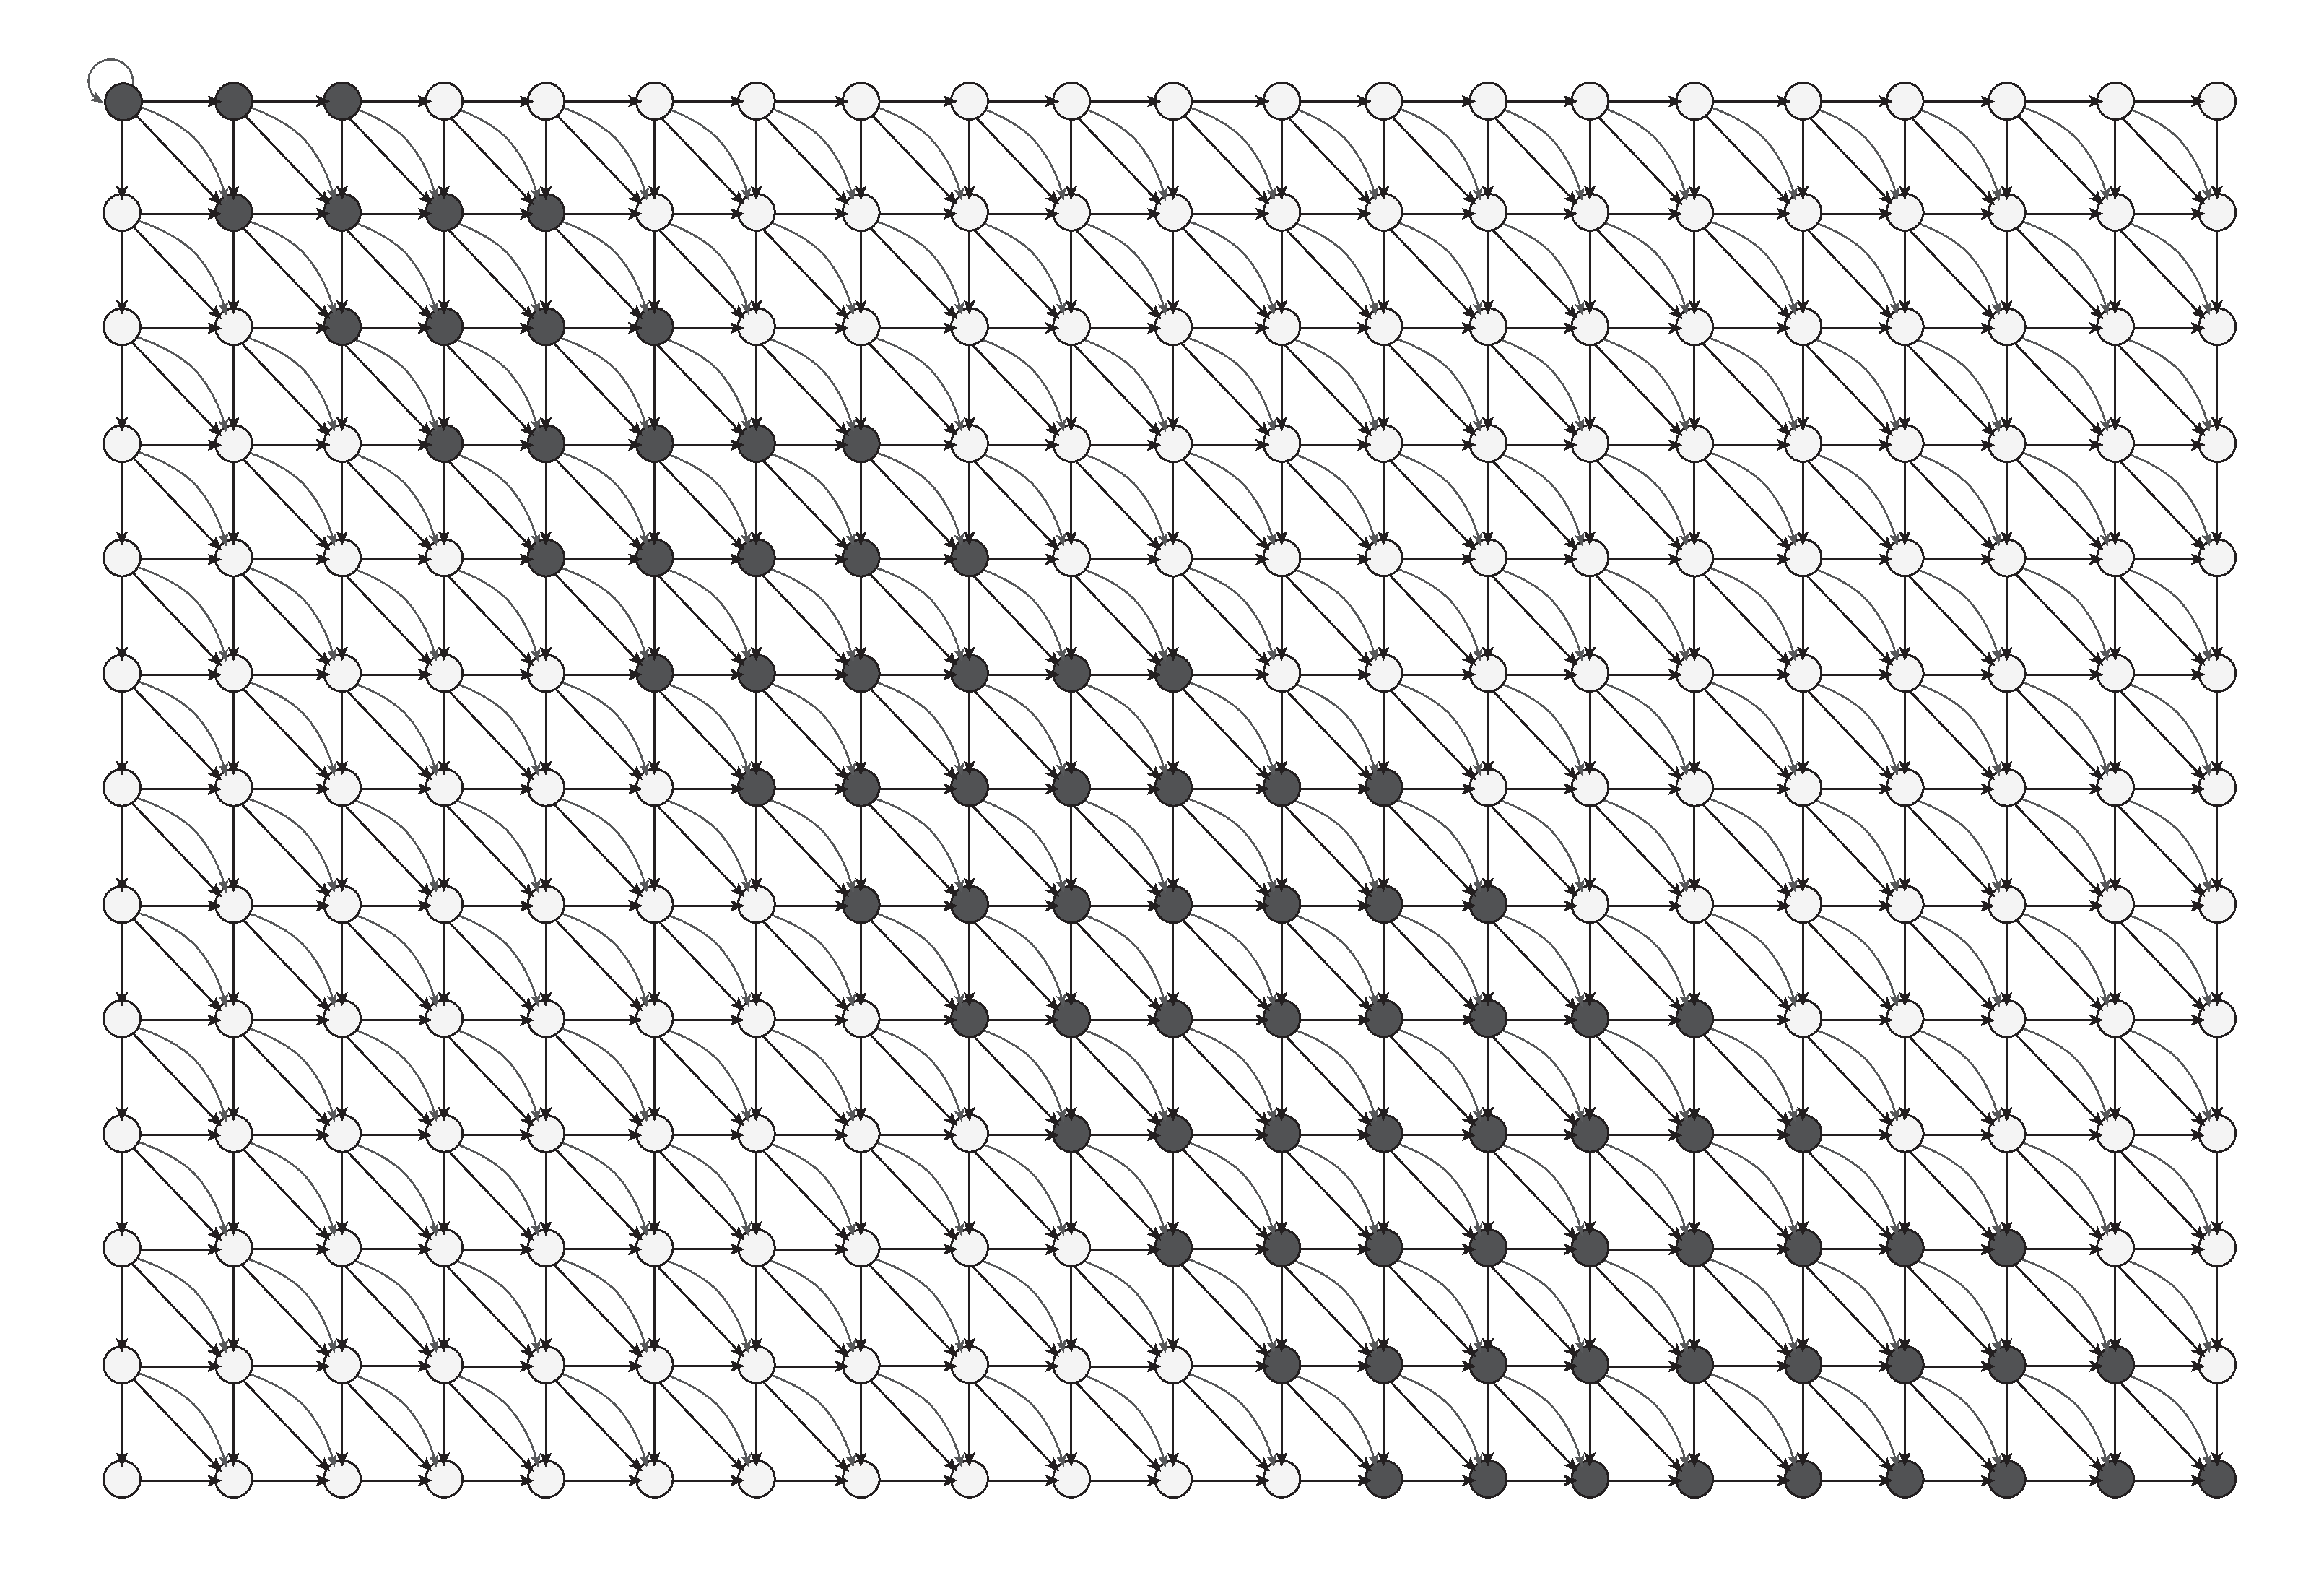
\includegraphics[scale=0.65]{sparsity_of_the_DFA.pdf}}
\caption{The Levenshtein automaton of Seeq is sparse. The sketch
represents the edit graph for a pattern of length 25 with 12
tolerated errors. The dark dots cover a region where active
states are approximately 95\% of the time. This region is
substantially smaller than the full edit graph and contains
221,930 different DFA states.
}\label{sparsity}
\end{figure}

Computing the number of states in this region in general terms is
not trivial, however in the example above there are 221,930 states
\textit{i.e.} less than one millionth of the upper bound $3^{25}$.
In reality, active states are not independent, so this sketch
only has a heuristic value. The upshot is that the DFA will spend
most of its time in a small number of states, and the probability
that other states are visited is low. Biological sequences are
not random streams, but their structured and repeated nature will
reduce the number of visited states rather than increase it.

\section{Performance}

The key (and underappreciated) strength of Seeq is that the number
of states visited by a Levenshtein automaton is much lower than
expected. The immediate consequences are that the memory won't blow
up and that you will rarely use dynamic programming. Most of the
time, Seeq just follows pointers, and because lazy DFAs have good
locality [1], many of those are cache hits.

Upon reading the reviewers comments, we realized that the benchmark
shown in the manuscript is not convincing. Our bad. We hope that
we can do better in this response in order to give a feel for the
performance of Seeq. Reviewer 2 suggested to benchmark Seeq against
Myer's bitvector algorithm, SeqAn and Razers3. SeqAn is a very high
quality library, but it takes some time to get familiar with, so we
are still not proficient to write competitive software with it.

In what follows we search approximate matches of sequences of length 20,
27, 34 and 42 in the humgan genome. All the sequences are prefixes of
the random sequence \texttt{GATGTAGCGCGATTAGCCTGAAAATGCGAGTACGGCGCGAAT}.
The input is a fasta file of hg19 (sequences were downloaded from [8],
concatenated and every chromosome was put on a single line). The
software was run on a 16-core dual-processor Intel Xeon with 256 GB
of DDR3-RAM at 1,866 MHz and a solid state hard drive.

The running time of the naive implementation of Myer's bitvector
algorithm (\textit{i.e.} as provided in [4]) ran between 47 and 50
minutes. As expected from the conditions of our benchmark, the running
time is nearly constant. However, this is far from competitive, as
can be seen in Table~\ref{benchmark}. The running time of Razers3
ranged from 53 seconds to ~6 minutes, and that of Seeq from 10 seconds
to ~3 minutes. On many of these problems, Seeq ran faster than
the Linux \texttt{wc} command (30 seconds), which only counts
characters. Seeq is about five times faster than Razers3 in full
sensitivity mode and two to five times faster than Razers3 in 99\%
sensitivity mode.

\begin{table}[h]
\centering
\begin{tabular}{c|c||c|c|c|c||c|c}
  \multicolumn{2}{c}{} & \multicolumn{4}{c}{Seeq} &
      \multicolumn{2}{c}{Razers3} \\
  \hline
  m  & k & time (s) & \# hits & mem (MB) & DP (s) & time (s) & \# hits \\
  \hline
  20 & 3  & 10  & 58     & 0.11    & 0.00 & 53/53 & 58/58 \\
  20 & 4  & 10  & 2908   & 0.46    & 0.00 & 76/77 & 2908/2908 \\
  20 & 5  & 10  & 68566  & 1.45    & 0.03 & 82/106 & 63803/68647 \\
  27 & 3  & 10  & 0      & 0.10    & 0.00 & 61/61 & 0/0 \\
  27 & 4  & 10  & 0      & 0.32    & 0.02 & 64/69 & 0/0 \\
  27 & 5  & 10  & 29     & 0.95    & 0.04 & 59/96 & 23/29 \\
  27 & 6  & 11  & 552    & 2.70    & 0.06 & 99/199 & 550/552 \\
  27 & 7  & 14  & 8795   & 7.76    & 0.19 & 98/201 & 8622/8796 \\
  27 & 8  & 17  & 107809 & 21.9    & 0.54 & -/205 & -/107909 \\
  34 & 5  & 10  & 0      & 0.94    & 0.02 & 63/67 & 0/0 \\
  34 & 6  & 11  & 0      & 2.48    & 0.10 & 79/108 & 0/0 \\
  34 & 7  & 13  & 1      & 5.83    & 0.24 & 68/102 & 1/1 \\
  34 & 8  & 19  & 37     & 13.10   & 0.50 & 120/247 & 37/37 \\
  34 & 9  & 23  & 527    & 28.22   & 1.04 & 120/256 & 524/527 \\
  34 & 10 & 29  & 6797   & 50.51   & 2.26 & -/252 & -/6798 \\
  42 & 8  & 17  & 0      & 13.92   & 0.57 & 66/73 & 0/0 \\
  42 & 9  & 23  & 0      & 29.91   & 1.34 & 65/123 & 0/0 \\
  42 & 10 & 30  & 1      & 61.20   & 2.39 & 122/340 & 1/1 \\
  42 & 11 & 39  & 6      & 121.47  & 5.14 & 126/344 & 6/6 \\
  42 & 12 & 53  & 52     & 232.71  & 9.30 & 123/347 & 52/52 \\
  42 & 13 & 75  & 772    & 424.35  & 18.06 & -/352 & -/772 \\
  42 & 14 & 109 & 8664   & 738.23  & 32.17 & 46/46 & 0/0 \\
  42 & 15 & 161 & 82507  & 1260.50 & 55.44 & 46/46 & 0/0 \\
  42 & 15 & 177 & 82507  & 555.91* & 71.58 \\
\end{tabular}
\caption{Benchmark of Seeq against Razers3. We searched patterns of
length 20 to 42 (parameter m) with errors ranging from 3 to 15
(parameter k) in the human genome (a fasta file of hg19). For Seeq
we recorded the running time, the number of hits discovered, the
memory usage of the DFA and the time spend in dynamic programming.
For Razers3, we recorded the running time and the number of hits
discovered. The first number was obtained by using the default sensitivity
\texttt{-rr 99} and the second by using the maximum sensitivity 
\texttt{-rr 100}. In the last case, Seeq was run with the option
\texttt{-y500} to limit the memory usage to 500 MB, which is why
the memory usage is marked by a star. Note that Seeq does not
allow overlapping matches while Razers3 does, which explains that
the number of hits can be different. A dash (-) indicates that
Razers3 crashed with segmentation fault.
\label{benchmark}
}
\end{table}

We also recorded the memory usage of Seeq. The most difficult problem
requested over 1.2 GB of RAM, but limiting the memory to ~500 MB
increased the running time by only 9\%. Also notice that the
memory footprint did not exceed 22 MB for patterns of 27
nucleotides, which is an empirical confirmation of the heuristic
argument above that the number of visited states is insignificant
compared to the worst-case estimates.

The last indicator that we collected is the time spent in dyamic
programming. Except for the most difficult problems, this number
does not exceed 10\% of the total running time, which means that
in many cases, the user could not notice any increase in speed even
if we made this step instantaneous. It is important to realize that
even on the most difficult problems, dynamic programming is performed
very few times. To give a figure, this happens once every 368
nucleotides in the last problem of Table~\ref{benchmark} (and once
every 1.6 million nucleotides in the first). Only when searching
long patterns with high error rates would it pay off to use
modern hardware to accelerate dynamic programming. But long patterns
with high error rates is the turf of other algorithms (for instance
BLAST).

We also noticed that Razers3 crashed on the most difficult problems
or even failed silently. We will get in contact with the maintainers
about this issue. Also, we would like to point out that Razers3 is
a mapper, so performing the benchmark with only one sequence
at a time is not showing its true potential. We used it in this
condition to better highlight the differences of the algorithms
running in the background, but we do not claim that Seeq is a point
blank replacement of Razers3.


\begin{figure}[!tpb]
\centerline{\includegraphics[scale=.90]{run_course.pdf}}
\caption{Processing course of a Seeq run. The line represents the
time required to process the given amount of input on the last
problem shown in Table~\ref{benchmark} (without memory limit).
Notice the run is slowest at the beginning and reaches its steady
state after ~10\% of the input has been processed.
}\label{course}
\end{figure}

Finally, we wish to highlight a key property of Seeq and lazy DFAs.
Fig.~\ref{course} shows a processing course on the last
problem of Table~\ref{benchmark} (without memory limit). As expected,
the run is slow at the beginning and only achieves a steady state
speed after ~10\% of the input has been processed, which is about
300 MB. Remember that lazy DFAs were initially benchmarked on much
smaller files, which explains that their performance was only
slightly better, if not worse than other algorithms.


\section{Conclusion}

Lazy DFAs have been analyzed at a time when they had mostly a
theoretical interest. They can be implemented efficiently on
modern hardware where their advantage over other algorithms
increases with file size. The core engine of Seeq is not novel,
it is actually an antique. And yet its performance is unmatched
for the reasons explained above.

We believe that this message is important for the bioinformatics
community. Not only because Seeq is useful, but because
lazy DFAs will have applications in many problems.

\section{Now what?}

Retrospectively, we agree that the manuscript was weak and rejecting
it was the right decision. Because of the two-page limit, we opted
to write it from the perspective of the user and missed major points
about the relevance of lazy DFAs for modern problems. Yet, we
believe that Seeq is useful and that it carries a simple and important
message for modern bioinformatics. This is why we ask the permission
to submit another version of the manuscript. Here is a summary of
that actions that we may take at this stage.

\vspace{.2in}

\noindent
\textbf{What we will do}.
\noindent
Regardless of what happens to this submission, we will
\begin{enumerate}
\item Write a complete documentation in pdf format.
\item Improve the code as per the comments of reviewer 1.
\item Rewrite the manuscript completely.
\item Change the benchmark as indicated by reviewer 2.
\end{enumerate}

\noindent
\textbf{What we will not do.}
\noindent
For the reasons explained above, we will not
\begin{enumerate}
\item Use vectorization to speed up dynamic programming.
\end{enumerate}

\noindent
\textbf{What we may do.}
\noindent
Depending on the decision about the manuscript and how
much the following is justified, we may
\begin{enumerate}
\item Write a full rebuttal. We will of course write a
formal rebuttal if this work is considered for
publication.
\item Paralellize the algorithm. This is possible only when
searching multiple patterns, which is not the core job of
Seeq.
\item Implement tunable costs and affine gaps. In this
case the threshold distance is less meaningful for the
user, but we can do it if some applications require it.
\end{enumerate}


\section{References}

[1] https://swtch.com/~rsc/regexp/regexp1.html
\par\noindent
[2] http://blog.notdot.net/2010/07/Damn-Cool-Algorithms-Levenshtein-Automata
\par\noindent
[3] A guided tour to approximate string matching. Navarro, Gonzalo.
ACM computing surveys (CSUR), 2001
\par\noindent
[4] A fast bit-vector algorithm for approximate string matching based
on dynamic programming. G Myers - Journal of the ACM (JACM), 1999
\par\noindent
[5] Finding approximate patterns in strings. E Ukkonen - J. Algorithms,
1985.
\par\noindent
[6] Approximate string matching by finite automata. Melichar, Bořivoj.
Computer Analysis of Images and Patterns. Springer Berlin Heidelberg, 1995.
\par\noindent
[7] Approximate text searching. PhD thesis, Depat. of Computer Siences,
University of Chile, December 1998. pp. 118-124.
\par\noindent
[8]http://hgdownload.cse.ucsc.edu/goldenpath/hg19/chromosomes/

\end{document}
